\subsection{Resultado}
Observando as métricas relevantes ao \textit{Earned Value Management} vemos que o \textit{Actual Cost} é igual ao \textit{Earned Value} mostrando que o projeto tem o custo controlado, por outro lado vemos que o Planed Value é superior ao Earned Value significando um atraso.

O \textit{MS Project} permite visualizar que a estimativa se mantém, como esperado.

Com estes atrasos e com o respetivo progresso tido até ao momento, é possível verificar que na realidade possuimos não 25\% como realmente pretendiamos concluido uma vez que a estratégia usada era uma divisão de atividades e não de durações. Assim verifica-se que na realidade ao invés do valor anteriormente referido, verifica-se que 38\% do projeto se encontra já concluido, em metade da duração, claro devido ao atraso propositado.

\begin{center}
    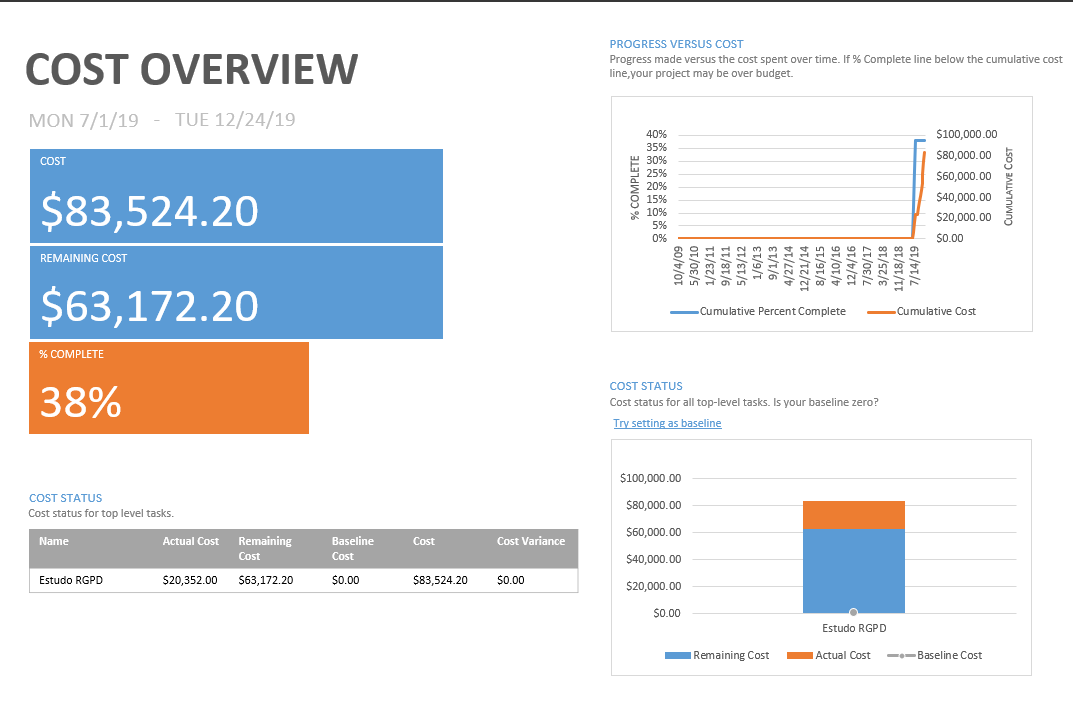
\includegraphics[width=0.7\textwidth]{media/baseline2CostOverview.PNG}
    \captionof{figure}{\textit{Baseline 2} - \textit{Cost Overview}}
\end{center}

Relativamente aos recursos, é visível quais se encontram usados até ao momento, quantidade dos mesmos restante e os respetivos custos, sempre atualizados.

\begin{center}
    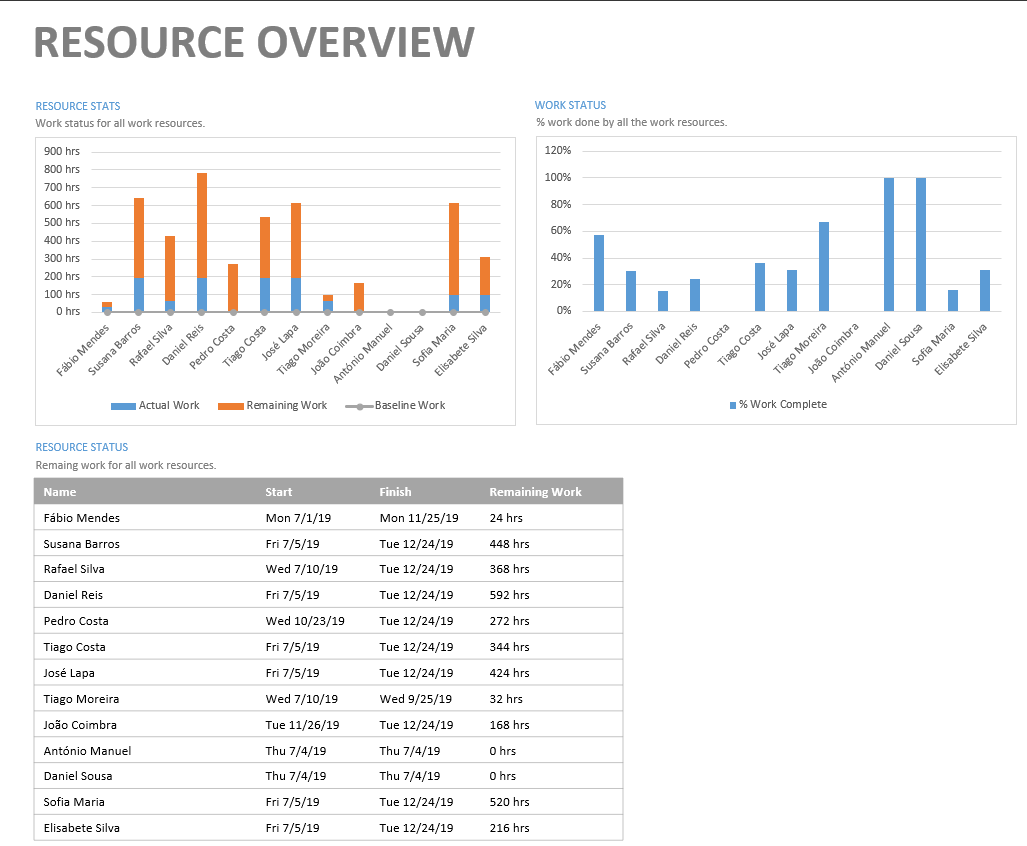
\includegraphics[width=0.7\textwidth]{media/baseline2ResourceOverview.PNG}
    \captionof{figure}{\textit{Baseline 2} - \textit{Resoursce Overview}}
\end{center}

\begin{center}
    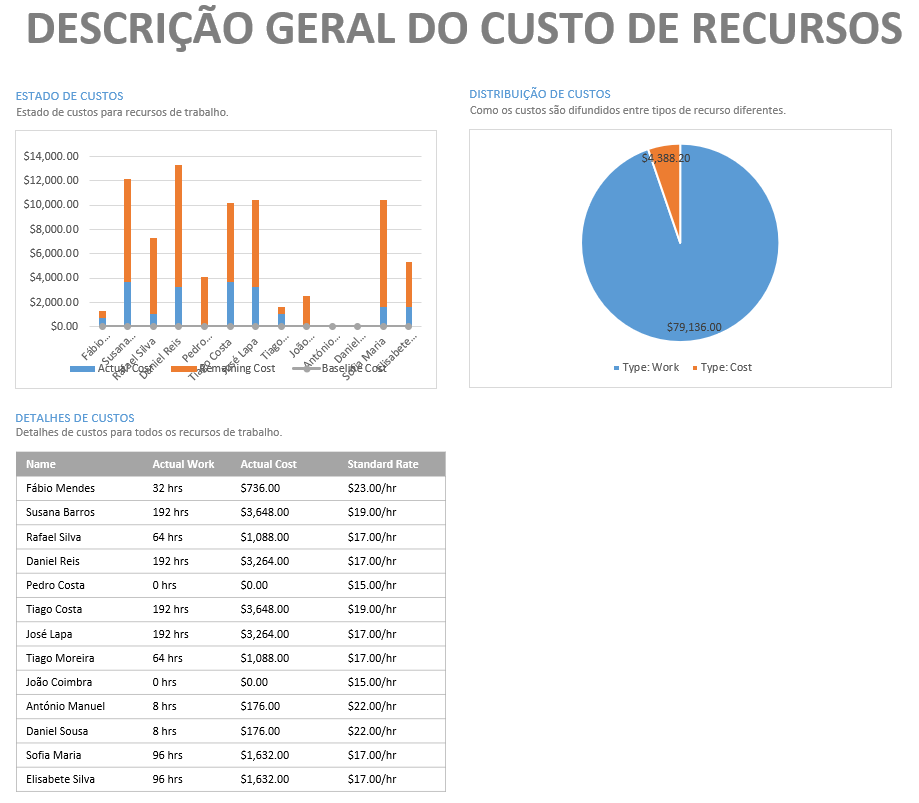
\includegraphics[width=0.7\textwidth]{media/baseline2ResourcesCost.PNG}
    \captionof{figure}{\textit{Baseline 2} - \textit{Resource Cost}}
\end{center}

Na imagem seguinte é possível visualizar que o \textit{Earned Value} calculado automaticamente pelo \textit{Microsoft Project} é de 23,288.60\$, quando na realidade o esperado seria 31,739.20\$, recorrendo à fórmula $EV = \textit{Complete Percentage} * \textit{Budget} $

\begin{center}
    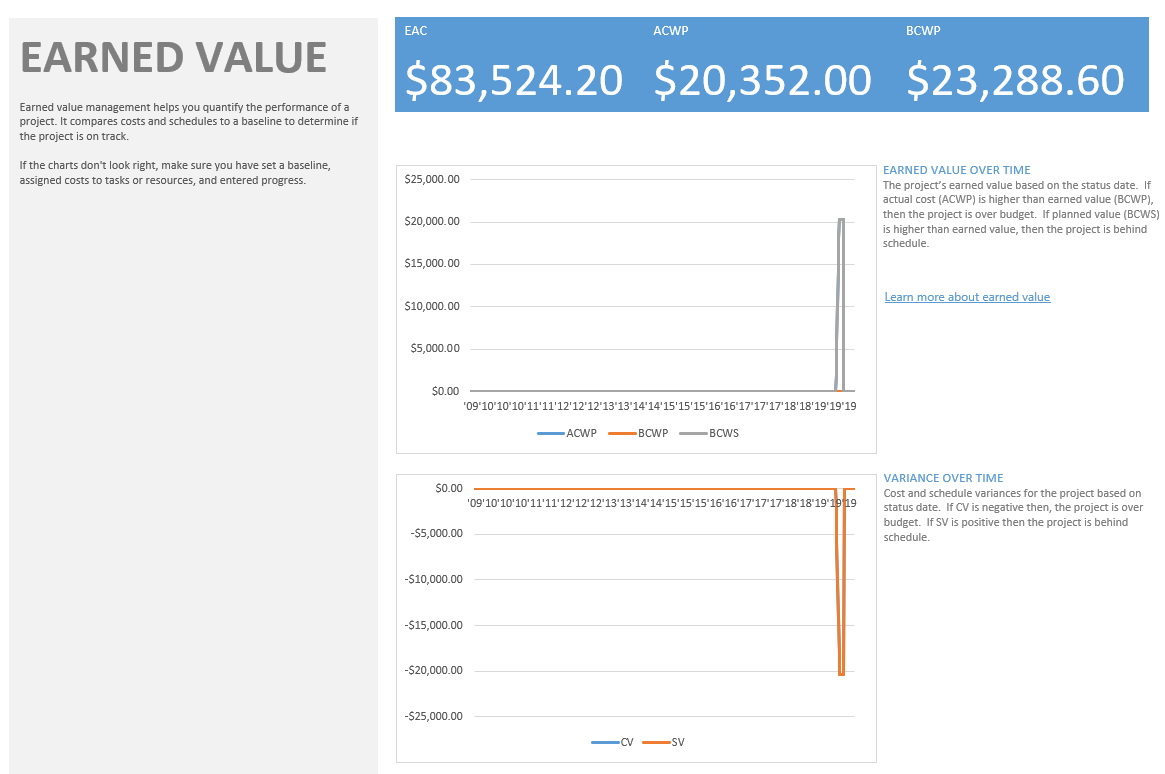
\includegraphics[width=0.8\textwidth]{media/baseline2EarnedValue1.PNG}
    \captionof{figure}{\textit{Baseline 2} - \textit{Earned Value 1/2}}
\end{center}
\begin{center}
    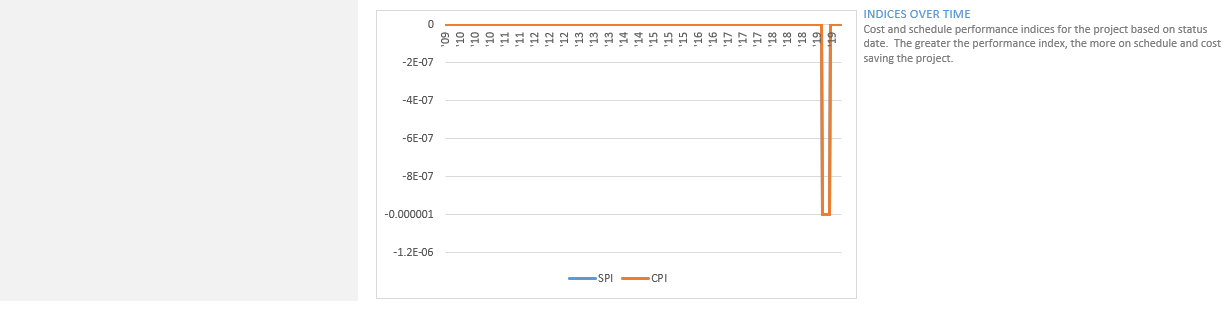
\includegraphics[width=0.8\textwidth]{media/baseline2EarnedValue2.PNG}
    \captionof{figure}{\textit{Baseline 2} - \textit{Earned Value 2/2}}
\end{center}